\documentclass[a4paper,11pt]{style-esi/td}

\usepackage{style-esi/licence}
\usepackage{style-esi/exercice}
\usepackage{style-esi/listing}
\usepackage{style-esi/tutoriel}
\usepackage{style/dev1}

\begin{document}

\seance{9}{Les tests unitaires}{td09-tests-unitaires}{
	Un code est souvent modifié. Cela veut dire que le temps passé à le
	simplifier permet souvent un gain de temps lors d’une modification
	ultérieure.  Il est même parfois conseillé de~:  écrire un code simplement
	fonctionnel, de le modifier afin d'améliorer sa lisibilité et sa modularité
	et, enfin, d'améliorer son efficacité.

	Toutes ses modifications du code imposent que le code soit testé. Il doit
	être testé à chaque modification ce qui serait fastidieux si les tests
	n'étaient pas automatisés.  Heureusement, c'est ce que propose JUnit.
}

%====================
\section{Introduction}
%====================	

La démarche que l'on vous propose de suivre dans ce TD permet de limiter au maximum
le nombre de \textit{bugs} dans son code%
\footnote{%
	Un code sans bug est difficile à obtenir,
	mais un développeur doit les éviter autant qu'il peut.
}.

Les tests unitaires ainsi que le développement dirigé par les tests permettent
d'obtenir des tests maintenables tout au long de la vie d'un code et
d'atteindre l'objectif d'un code (quasi) exempt de \textit{bugs}.

Jusqu'à présent, nous avons écrit du code afin de répondre à une demande.
Pour cela, il a fallu~:
\begin{enumerate}
	\item lire et comprendre l'énoncé~;
	\item déterminer les entrées et les sorties~;
	\item penser votre algorithme~;
	\item construire l'algorithme puis l'écrire en Java~;
	\item tester votre algorithme.
\end{enumerate}

Ce laboratoire présente le \emph{développement dirigé par les tests}.
Pour faire court, il s'agit d'écrire les tests avant d'avoir écrit le code.
Cela est possible car on sait, avant de l'écrire, ce que le code est censé faire.

La démarche est la suivante~:
\begin{enumerate}
	\item lire et comprendre l'énoncé~;
	\item déterminer les entrées et les sorties~;
	\item penser aux tests que vos méthodes devront passer~;
	\item écrire les tests~;
	\item penser votre algorithme~;
	\item construire l'algorithme puis l'écrire en Java~;
	\item tester votre algorithme.
\end{enumerate}

%====================
\section{La couverture de code}
%====================	

Ensemble, tentons de comprendre ce qu'est une bonne \emph{couverture de code}
en reprenant notre fonction valeur absolue qui est définie de la façon suivante~:
$$
	|x| = x \textrm{ si } x \geq 0, -x \textrm{ sinon}.
$$

Soit la méthode \texttt{abs} qui a pour signature
\code{java}{public static double abs(double x)}.

Nous allons maintenant réfléchir aux tests que nous devons réaliser
afin de garantir le bon fonctionnement de cette méthode.
C'est-à-dire, les tests nécessaires%
\footnote{%
	Avoir les tests nécessaires et suffisants c'est mieux.
	À défaut, il en vaut mieux trop que pas assez.
}
pour garantir le fonctionnement de la méthode
quelle que soit l'entrée passée à la méthode.

Prenons une valeur positive, 4 par exemple.
Le code suivant, qui est pourtant faux,
passe avec succès notre test puisqu'il va retourner la valeur d'entrée.
\begin{Code}{Java}
	public static double abs(double x) {
		return x;
	}
\end{Code}

Notre test pourrait faire croire que la méthode est correcte.
Ce qui montre bien que notre batterie de tests est insuffisante.

Ajoutons un second test en essayant l'entrée $-4$.
Le code suivant, qui n'est pas la valeur absolue, passe avec succès nos deux tests.

\begin{Code}{Java}
	public static double abs(double x) {
		return 4;
	}
\end{Code}

Si nous prenons toutes nos observations en considération,
nous obtenons le plan de tests suivant~:

\begin{center}
	\begin{tabular}{|c|c|c|c|}
		\hline
		\no du test & entrées & résultat attendu & note           \\
		\hline
		1           & 4       & 4                & nombre positif \\
		\hline
		2           & -7      & 7                & nombre négatif \\
		\hline
	\end{tabular}
\end{center}

Même si notre exemple est aberrant,
nous souhaitons ici mettre en évidence la difficulté d'obtenir des tests complets,
que le processus d’élaboration des tests unitaires demande de la réflexion
et qu’il ne garantit pas à 100\% le bon fonctionnement du code.
Il est donc essentiel de prendre le temps nécessaire
afin de fournir une couverture de code aussi complète et exacte que possible%
\footnote{%
	Vous pouvez remarquer que pour chacun de nos exemples,
	la couverture de code est de 100\% ;
	et que malgré cela, le code ne fait pas toujours ce qu'on souhaitait qu'il fasse.
}.

\begin{Exercice}{Max - Couverture de code}
	Donnez les entrées et sorties nécessaires à l’élaboration d’une bonne
	couverture de code pour la méthode \code{java}{max(int a, int b)} qui
	permet d’obtenir la plus grande valeur parmi les~2 passées en
	paramètre.
\end{Exercice}

\begin{Exercice}{Somme d'entiers consécutifs - Couverture de code}
	Donnez les entrées et sorties nécessaires à l’élaboration d’une bonne couverture de code pour la méthode \code{java}{somme(int n)}. Cette méthode calcule la somme des entiers consécutifs de 1 à n.
\end{Exercice}

\begin{Exercice}{Anagramme - Couverture de code}
	Donnez les entrées et sorties nécessaires à l’élaboration d’une bonne couverture de code de la méthode \code{java}{boolean estAnagramme(String mot, String candidat)}. Cette méthode vérifie si une chaîne de caractères est une anagramme.
	\begin{quote}
		\og Une anagramme est une construction fondée sur une figure de style qui inverse ou permute les lettres d’un mot ou d’un groupe de mots pour en extraire un sens ou un mot nouveau.\fg
		Wikipedia\footnote{https ://fr.wikipedia.org/wiki/Anagramme}.
	\end{quote}
\end{Exercice}

\begin{Exercice}{Palindrome - Couverture de code}
	Donnez les entrées et sorties nécessaires à l’élaboration d’une bonne couverture de code de la méthode \code{java}{boolean estPalindrome(String mot)}. Cette méthode vérifie qu'un texte est un palindrome.
	\begin{quote}
		\og Le palindrome est un texte ou un mot qui reste identique qu’on le lise de gauche à droite ou de droite à gauche. Nous considérons ici la version stricte dans le sens où l’on prend en considération les signes diacritiques (accents, trémas, cédilles) ainsi que les espaces.\fg{} Wikipedia\footnote{https ://fr.wikipedia.org/wiki/Palindrome}.
	\end{quote}
\end{Exercice}

\begin{Exercice}{Nombre occurrences - Couverture de code}
	Donnez les entrées et sorties nécessaires 
	à l’élaboration d’une bonne couverture de code 
	de la méthode \code{java}{public static int nbOccurences(char lettre, String texte)}. 
	Cette méthode permet de compter le nombre d'occurrences d’une lettre dans un texte.
\end{Exercice}

%====================
\section{JUnit}
%====================

Si nous reprenons l’exemple de la méthode calculant la valeur absolue, nous pourrions la développer et la tester comme ceci :
\listing[basicstyle=\footnotesize\vtt]{java}{MonMath.java}

Au lancement du code, les deux tests passent.
\begin{Console}
	abs(4) = 4 ? true
	abs(-6) = 6 ? true
\end{Console}

Les problèmes avec cette méthodologie sont multiples.
\begin{enumerate}
	\item Il ne peut y avoir qu’une seule méthode main par fichier Java.
	\item Il faut être rigoureux pour que les tests soient lisibles.
	\item Il faut vérifier à l'écran que chaque ligne affiche un \samp{true}
	      ce qui peut prendre du temps s'il y a des centaines de tests.
	\item Le lancement des tests peut prendre du temps
	      puisqu'il faut lancer chaque fichier séparément\dots
\end{enumerate}

Tous ces problèmes mènent à un problème de maintenabilité des tests et du code.

Notre manière de tester peut être améliorée
en sortant les méthodes principales dans des fichiers différents
et le dernier point en mettant tous les tests dans la même méthode,
mais il nous reste à être rigoureux pour obtenir un code maintenable.
Nous allons donc utiliser le framework \bsc{JUnit}
qui va nous permettre d'obtenir cette lisibilité.

\subsection{Écrire des tests unitaires}
%---------------------------------------

La première chose à faire est de configurer \bsc{Netbeans}.
Heureusement pour vous, il fait presque tout lui même (à condition de bien s’y prendre).
Après avoir écrit le fichier \samp{MonMath.java} dans un nouveau package
\samp{esi.dev1.td9}, faite un clic droit sur la classe à tester.
Sélectionnez tools et faites \textit{Create/Update tests}.

\begin{figure}[hbt!]
	\begin{center}
		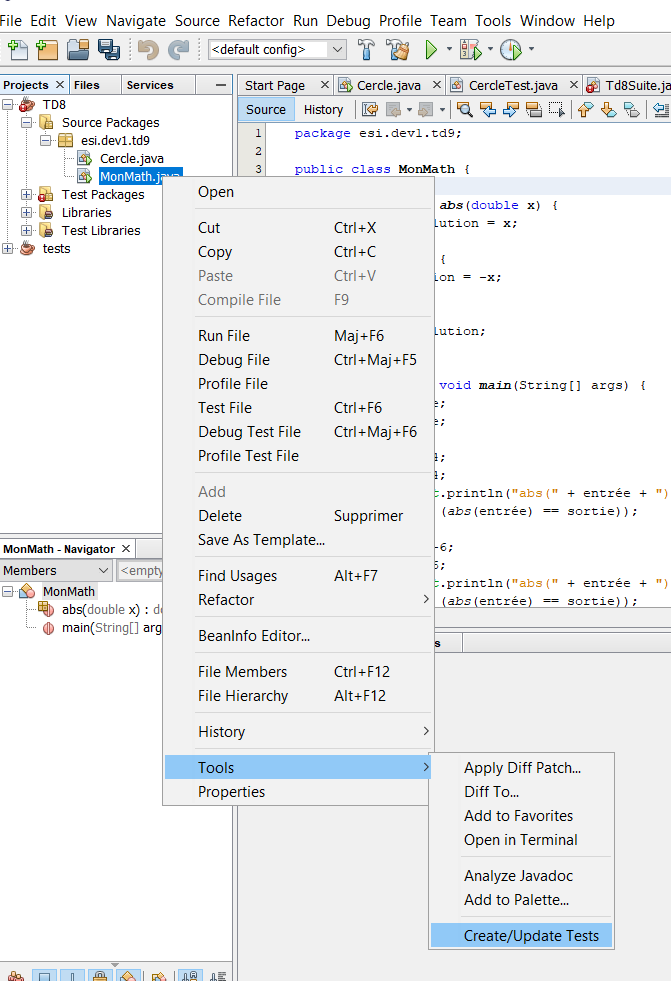
\includegraphics[width=.4\textwidth]{images/create_tests}
	\end{center}
	\caption{Demande de création des tests}
\end{figure}

Une nouvelle fenêtre va apparaître, décochez les 4 \textit{checkbox} en
dessous de \textit{Generated Code} et validez.

\begin{figure}[hbt!]
	\begin{center}
		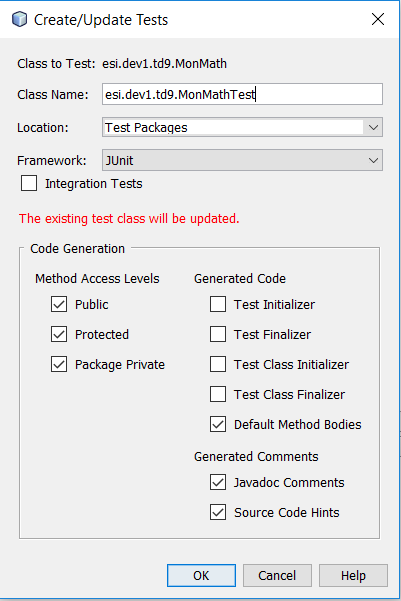
\includegraphics[width=.3\textwidth]{images/config_tests}
	\end{center}
	\caption{Choix des tests qui seront créés automatiquement}
\end{figure}

De nouveaux éléments, créés par \bsc{Netbeans}, apparaissent dans votre projet.
Remarquez un nouveau dossier nommé \emph{Tests packages}
dans lequel se trouve une nouvelle classe \texttt{MonMathTest.java}.
C'est dans cette classe que vous écrirez vos premiers tests.

\begin{figure}[hbt!]
	\centering
	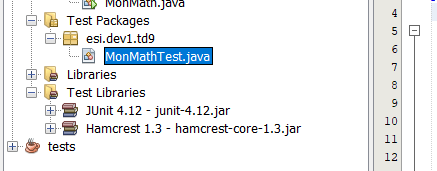
\includegraphics[width=.4\textwidth]{images/libraries}
	\caption{Montre l'arborescence créée}
\end{figure}

Il vous reste à considérer le message laissé par NetBeans et compléter le code.
\begin{Code}{Java}
	// TODO review the generated test code and remove the default call to fail.
\end{Code}

Une fois le code ajouté, vous devriez obtenir ceci~:
\listing{java}{MonMathTestEMPTY}

La variable x représente l’entrée de la méthode à tester
et la variable \texttt{expResult} représente le résultat attendu.

La méthode \texttt{asserEquals} est une méthode qui prend en paramètre :
\begin{itemize}
	\item le résultat attendu~;
	\item le résultat obtenu (calculé par la méthode que vous souhaitez tester)~;
	\item une marge d’erreur.
\end{itemize}

Le troisième paramètre ne doit être utilisé
que si la sortie de la méthode est de type pseudo-réel, dans ce cas \samp{double}%
\footnote{Pourquoi ?}.
L’appel à la méthode \samp{assertEquals} avec un retour de méthode entier
s’écrit donc : \code{java}{assertEquals(expResult, result)}.

Si la méthode que vous testez retourne un booléen,
il est alors préférable d’utiliser les méthodes \code{java}{assertTrue(result)}
ou \code{java}{asserFalse(result)}.
Ces méthodes prennent un unique paramètre puisque le résultat attendu est défini
par le nom même de la méthode utilisée.

\subsection{Lancer les tests}
%----------------------------

Pour lancer les tests,
il suffit de choisir \texttt{Run/Test Project (Alt+F6)} dans le menu.
Vous pouvez également lancer un seul fichier de test
via un clic droit sur le fichier puis \texttt{Test File}.

\bsc{Netbeans} affiche alors un message
indiquant le nombre de tests lancés/réussis.

En cas d'erreur,
il génère un petit rapport reprenant pour chaque test lancé :
\begin{itemize}
	\item Son nom;
	\item La valeur attendue (expResult);
	\item La valeur obtenue.
\end{itemize}

\begin{infoit}{Un bon réflexe en cas d'erreur}
	Lorsqu'un test rate c'est parfois parce que le test a \textbf{mal été écrit}
	et pas à cause de la méthode testée. Soyez prudent !
\end{infoit}

\subsection{Bonnes pratiques}
%----------------------------

En cas d'erreur,
il faut pouvoir identifier rapidement ce qui n'a pas été et pourquoi.
Pour cela, le choix du nom  de la méthode de test est crucial.
Comme il ne sera jamais appelé explicitement,
il peut être très long !
Voici quelques exemples possibles pour le test de la valeur absolue d'un nombre positif.
\begin{itemize}
	\item \samp{testAbs\_nombrePositif}
	\item \samp{absQuandPositifAlorsInchangé}
	\item \samp{testAbs\_LaValeurDUnNombrePositifEstLuiMeme}
	\item \samp{abs\_NombrePositif\_ResteInchangé}
\end{itemize}

On peut aussi veiller à rendre le code du test le plus lisible possible.
Voici une écriture possible pour le test de la valeur absolue d'un nombre négatif.
\begin{Code}{java}
	@Test
	public void abs_QuandNégatifAlorsInversé() {
		assertEquals(6.0, Math.abs(-6), 0.001);
	}
\end{Code}

\subsection{Tester le lancement d'une exception}
%=============================

Voici le code d'une méthode qui calcule le périmètre d'un cercle.
\listing[linerange=11-16]{java}{Cercle.java}

Nous remarquons qu'une exception est lancée dans le cas d'un rayon négatif.
Un plan de tests devrait ressembler à~:

\begin{center}
	\begin{tabular}{|c|c|c|c|}
		\hline
		\no du test & entrées & résultat attendu & note                             \\
		\hline
		2           & 4       & 25.12            & valeur positive (précision 0.01) \\
		\hline
		1           & 0       & 0                & plus petite entrée acceptée      \\
		\hline
		3           & -5      & \texttt{erreur}  & valeur négative                  \\
		\hline
	\end{tabular}
\end{center}

Nous vous laissons écrire les deux premiers tests.

Pour vérifier le lancement d'une exception dans le cas du troisième test,
ajoutez un paramètre au tag \texttt{@Test}
spécifiant le type de l'exception attendue.
Comme ci-dessous~:

\listing[linerange=14-17]{java}{CercleTest.java}

Remarquez que dans le cas présent, vous ne devez pas ajouter de méthode \texttt{assert}\footnote{Pourquoi ?}.

\begin{Exercice}{Couverture de code - Exceptions}
	Pour chacun des exercices précédents, 
	vérifiez que vous avez bien pensé aux cas menant à des erreurs.
\end{Exercice}

\begin{Exercice}{Développement guidé par les tests}
	Pour les exercices 1 à 5 
	--~c'est-à-dire pour 
	\texttt{max}, \texttt{somme}, \texttt{estAnagramme}, 
	\texttt{estPalindrome} et \texttt{nbOccurrences}~--
	pour lesquels vous avez écrit la couverture de code~:
	\begin{itemize}
		\item écrivez la signature de la méthode 
			et retournez une valeur quelconque afin de rendre le code compilable ;
		\item développez, avec \bsc{JUnit}, 
			votre couverture de code écrite précédemment. 
			Il s'agit d'écrire plusieurs tests;
		\item lancez l'exécution des tests. 
			Cette exécution va signaler des erreurs 
			(puisque la méthode retourne une valeur quelconque) ;
		\item corrigez la méthode afin qu'elle complète les tests.
	\end{itemize}
\end{Exercice}

%====================
\section{Exercices supplémentaires}
%====================	

\begin{Exercice}{Implémentation - PGCD Plus grand commun diviseur}
	Selon le principe vu précédemment, 
	implémentez la méthode \code{java}{pgcd(int a, int b)} 
	qui retourne le pgcd de deux nombres.
\end{Exercice}

\begin{Exercice}{Implémentation - PPCM Plus petit commun multiple}
	Selon le principe vu précédemment, 
	implémentez la méthode \code{java}{ppcm(int a, int b)} 
	qui retourne le ppcm de deux nombres.
\end{Exercice}

\begin{Exercice}{Implémentation - Chiffrement par décalage}
	Selon le principe vu précédemment, 
	implémentez la méthode \code{java}{césar(String texte, int décalage)} 
	qui permet de retourner un texte chiffré selon le code de César%
	\footnote{%
		\url{https://fr.wikipedia.org/wiki/Chiffrement_par_décalage}
	}.
\end{Exercice}

\end{document}